% options:
% thesis=B bachelor's thesis
% thesis=M master's thesis
% czech thesis in Czech language
% slovak thesis in Slovak language
% english thesis in English language
% hidelinks remove colour boxes around hyperlinks

\documentclass[thesis=B,czech]{FITthesis}[2012/06/26]

\usepackage[utf8]{inputenc} % LaTeX source encoded as UTF-8

\usepackage{graphicx} %graphics files inclusion
% \usepackage{amsmath} %advanced maths
% \usepackage{amssymb} %additional math symbols

\usepackage{dirtree} %directory tree visualisation

\usepackage{subfig}

% % list of acronyms
% \usepackage[acronym,nonumberlist,toc,numberedsection=autolabel]{glossaries}
% \iflanguage{czech}{\renewcommand*{\acronymname}{Seznam pou{\v z}it{\' y}ch zkratek}}{}
% \makeglossaries

\newcommand{\tg}{\mathop{\mathrm{tg}}} %cesky tangens
\newcommand{\cotg}{\mathop{\mathrm{cotg}}} %cesky cotangens

% % % % % % % % % % % % % % % % % % % % % % % % % % % % % %
% ODTUD DAL VSE ZMENTE
% % % % % % % % % % % % % % % % % % % % % % % % % % % % % %

\department{Katedra \ldots softwarového inženýrství}
\title{Florbalový trenér}
\authorGN{Jakub} %(křestní) jméno (jména) autora
\authorFN{Olejník} %příjmení autora
\authorWithDegrees{Jakub Olejník} %jméno autora včetně současných akademických titulů
\supervisor{Ing. Josef Gattermayer}
\acknowledgements{Rád bych poděkoval Ing. Josefu Gattermayerovi za odborné vedení této práce a~trenérským kolektivům florbalových oddílů FbC Panthers a~AC Sparta Praha Florbal za spolupráci v~analytické části této práce.}
\abstractCS{Práce se zabývá vývojem mobilní aplikace pro tablety s~operačním systémem iOS, která si klade za cíl zjednodušit florbalovým trenérům přípravu florbalových tréninků a~cvičení. Uživatel, který aplikaci využívá, by se díky ní měl plně soustředit na obsah tréninkové jednotky nikoliv na formu, ve které ji zachytí, a~ve které ji bude následně prezentovat svým svěřencům.}
\abstractEN{The thesis deals with development of a mobile application for tablets with operating system iOS, which should simplify preparations of floorball trainings and exercises. User of this application should fully focus on the content of training unit, not the form in which it will be captured and then presented to his team.}
\placeForDeclarationOfAuthenticity{V~Praze}
\declarationOfAuthenticityOption{4} %volba Prohlášení (číslo 1-6)
\keywordsCS{florbal, trenér, trénink, iOS}
\keywordsEN{floorball, coach, training, iOS}

\begin{document}

% \newacronym{CVUT}{{\v C}VUT}{{\v C}esk{\' e} vysok{\' e} u{\v c}en{\' i} technick{\' e} v Praze}
% \newacronym{FIT}{FIT}{Fakulta informa{\v c}n{\' i}ch technologi{\' i}}

\begin{introduction}
	V~dnešním světě jsou informační technologie využívány téměř ve všech oblastech lidské činnosti, přesto se dají najít činnosti jimi nedotčené. Za takovou oblast se dají považovat mladé a~zatím neolympijské sporty, které často doplácí na podmínky amatérského prostředí. Velmi často ani špičkové oddíly nejsou schopny nabídnout svým hráčům dostatečně kvalitní zázemí. Aplikace vyvíjená v~rámci této práce by mohla tento nedostatek alespoň zmírnit.

	Toto téma jsem si zvolil na základě osobní zkušenosti a vědomí, že taková mobilní aplikace zatím neexistuje, a desktopové varianty za moc nestojí. Podobné názory jsem zaznamenal vždy když jsem na toto téma diskutoval s~jinými florbalovými trenéry. Jejich reakce na vznik takové aplikace byly vždy kladné, a proto si myslím, že navržená aplikace bude využívána a mohla by pomoci zvednout kvalitu florbalových tréninků.
\end{introduction}

\chapter{Cíl práce}
	Výsledkem práce by měl být funkční prototyp, kterým bude možné nahradit nyní využívané kreslicí tabule. Využitím tabletu se odstraní nutnost použití jiných kreslicích nástrojů, které nemusí být vždy dostupné, popř. jejich viditelnost na tabuli není dostačující. Dále elektronickou tabuli nelze umazat tak, aby na ní nebylo vysvětlované cvičení čitelné, v~případě umazání displeje jej lze snadno očistit.

	Naopak cílem práce není aplikace určená pro libovolné kreslení. Takovou aplikaci by samozřejmě bylo možné využít i pro výše zmíněné účely, nicméně podpora symboliky, které se mezi trenéry a hráči již nyní využívá, tvoří fundamentální základ celé aplikace a~je hlavním znakem, který tuto aplikaci odlišuje od ostatních, které ji mohou svým zaměřením připomínat.

	Vytvořená aplikace nemá podporovat veškerou funkcionalitu zmíněnou v~této práci, výsledná aplikace má poskytnout dobře fungující základ, který bude možné v~budoucnu rozšiřit i o~jiné než zde zmíněné funkce.

	Zároveň je důležité navrhnout odpovídající uživatelské rozhraní, které bude dostatečně jednoduché a intuitivní. Stejně tak rozhraní nesmí odporovat zvyklostem platformy iOS, aby se uživatel v~aplikaci neztratil již po prvním spuštění.

\chapter{Analýza a návrh}

	Na začátku práce byla provedena analýza problematiky. Byly zohledněny dobré i špatné vlastnosti již existujících aplikací nejen na iOS, ale i na OS Android a desktopových systémech. V~rámci analýzy bylo provedeno dotazníkové šetření na jehož základě, byl upraven seznam funkcí, které jsou, nebo budou implementovány. Na základě této analýzy vznikla specifikace požadavků, která bude v~této kapitole rozebrána.

\section{Analýza požadavků}

\subsection{Dotazníkové šetření}\label{sec:survey}

	V rámci analytické části práce jsem se rozhodl oslovit vybraný vzorek potenciálních uživatelů aplikace. Primárním cílem tohoto šetření byla především kontrola, zda se podařilo zaměřit se na opravdu důležité časti aplikace. Dalším z cílů bylo získání povědomí o podobných aplikacích, které již někdo za podobným účelem použil.

	Jednotlivé body dotazníku budou rozebrány v této kapitole. Pro analýzu zmíněných podobných aplikací je připravena samostatná kapitola (\ref{sec:competition}).

\subsubsection{Cílové věkové kategorie} \label{sec:target_group}

	Jak je patrné z grafu \ref{graph:category}, šetření prokázalo, že cílovou skupinou budou trenéři starších kategorií (starší žáci a výše) \-- u mladších kategorií jsou priority nastaveny jinak, než u těch starších. Mladší (popř. začínající) hráče je třeba naučit florbalové základy \-- postoj, držení hole, střela, přihrávka, což je nutné předvést, nikoli kreslit.

	\begin{figure}
		\centering
		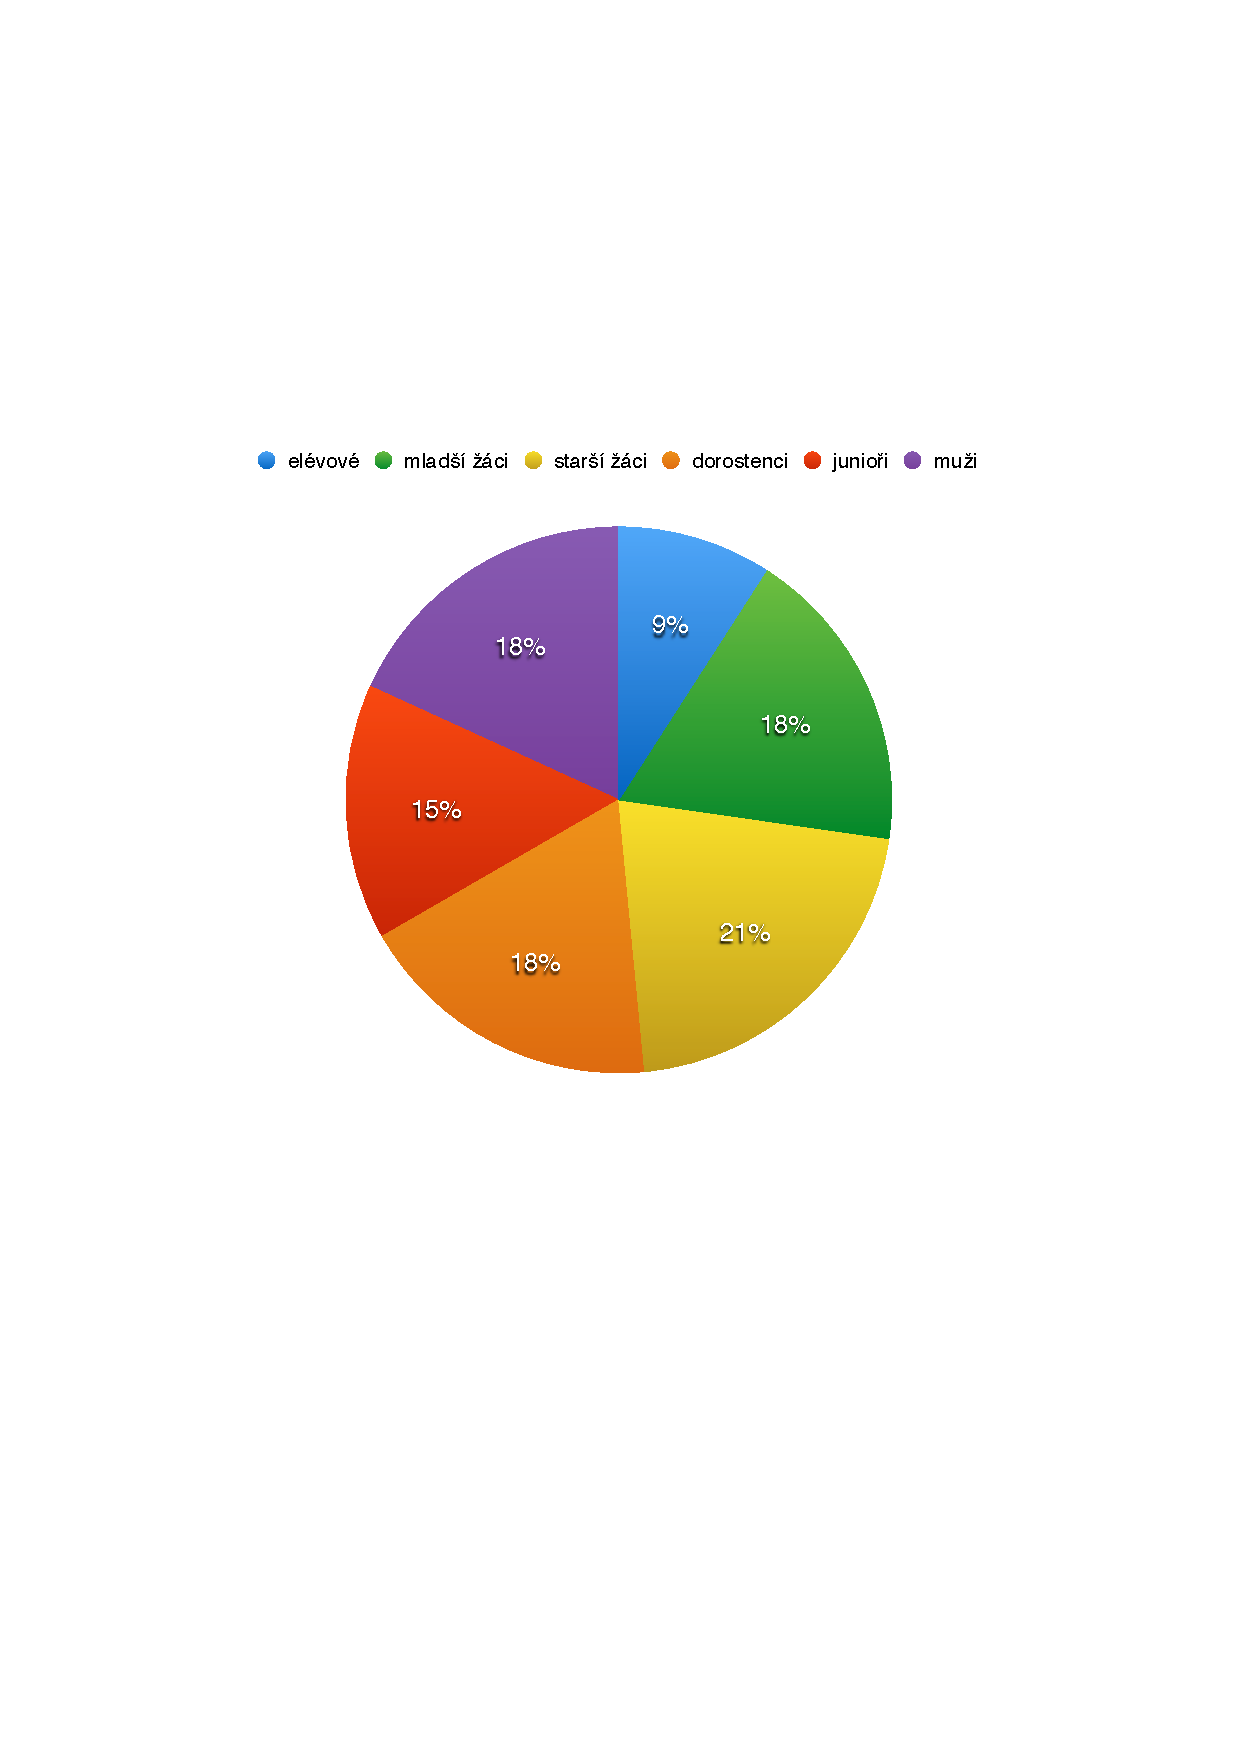
\includegraphics{img/graph_category}
		\caption{Graf trénovaných kategorií}\label{graph:category}
	\end{figure}

\subsubsection{Četnost užití kreslicí tabule}

	Dalším zjištěním (graf \ref{graph:table_usage}), které nebylo překvapením je fakt, že přibližně pouze pětina trenérů kreslicí tabuli nepoužívá vůbec, překvapením byla druhá část grafu \-- třetina trenérů ji využije více než pětkrát za trénink.

	Počet trenérů, kteří tabuli nevyužívají přibližně kopíruje počet trenérů, kteří trénují mladší kategorie, což potvrzuje tvrzení v předchozí kapitole (\ref{sec:target_group}).

	\begin{figure}
		\centering
		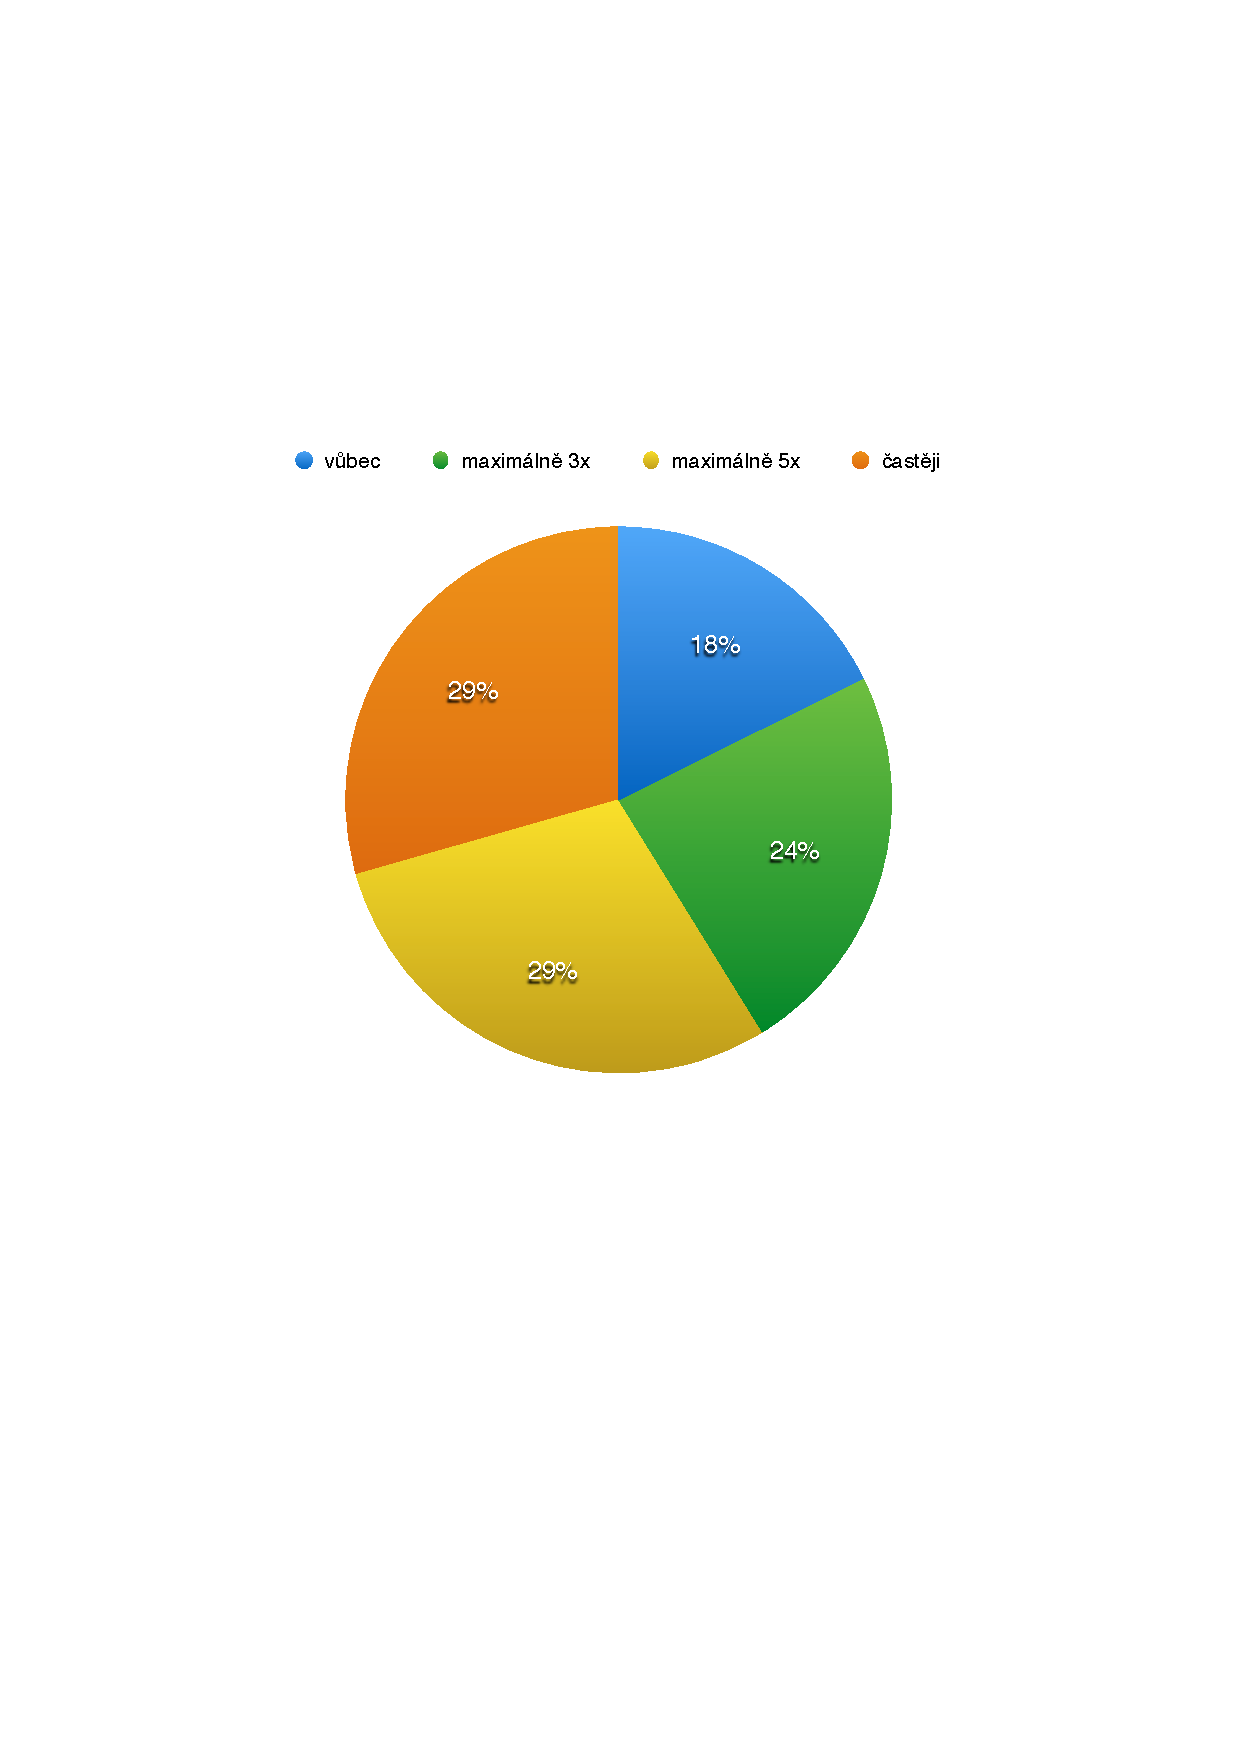
\includegraphics{img/graph_table_usage}
		\caption{Graf využítí kreslicí tabule}\label{graph:table_usage}
	\end{figure}

\subsubsection{Funkce volné kreslení, seskupování cvičení, perzistence}

	Výsledky potvrdily, že funkce volného kreslení (jako v Malování v MS Windows) je pro uživatele nepostradatelná. Toto od začátku měla být základní funkcionalita aplikace. Stejně zásadními se ukázaly funkce perzistentního uložení a funkce seskupování cvičení do tréninků. Seskupování bylo od začátku považováno za důležitou funkcionalitu, ale podle tohoto výsledku bylo rozhodnuto o jeho zařazení do aplikace.

\subsubsection{Textové poznámky}

	Naopak překvapením bylo, že textové poznámky nejsou pro trenéry tak důležité, třetina dotázaných by se bez nich obešla. Nicméně tato funkcionalita byla do aplikace zařazena, protože poznámkový aparát může sloužit jako upomínka pro trenéra, aby nezapomněl, co je důležité hráčům před cvičením zdůraznit, což vede k jejich růstu.

	Dalším důležitým faktorem je, že poznámky mohou do jisté míry nahradit funkcionalitu, která vyplynula z dotazníkového šetření jako chtěná (např. docházka), ale prozatím byla odložena. Tímto způsobem je možné ji nahradit bez časového zdržení a  implementačních komplikací.

\subsubsection{Automatické nakreslení cvičení}

	Zajímavou funkcionalitou, kterou by bylo dobré jednou v aplikaci mít, je automatické postupné nakreslení cvičení. Tato funkce snižuje nároky na prezentační schopnosti trenéra tím, že jednoduchým poklepáním je schopen připravené cvičení \uv{nakreslit}. Zároveň jsou sníženy nároky na grafické nároky na trenéra, protože nemusí ve spěchu a v nepohodlné pozici cvičení kreslit. Tato funkce se líbila všem dotázaným a je na seznamu funkcí, které budou do aplikace v nejbližší době doplněny. Takto bylo rozhodnuto z důvodu její pracnosti a omezené časové dotaci na tuto práci.

	Toto byl výčet původně navrhovaných funkcí, které by měly být v aplikaci implementovány, následující funkce jsou tipy, které by dotazovaní trenéři v aplikaci ocenili.

\subsubsection{Elektronická tužka}

	Jednou z navrhovaných funkcionalit je možnost vkládání videí a jejich následný rozbor, tzv. \uv{elektronická tužka}. Tato funkce bude z aplikace kompletně vynechána. Taková funkcionalita nepatří do aplikace tohoto typu, protože aplikace se zabývá přípravou cvičení a jeho případnému vysvětlení a elektronická tužka je poněkud jiného typu.

\subsubsection{Docházka}

	Další zmíněnou funkcí byla docházka na trénink. Tato funkce nebude implementována, protože nesouvisí s přípravou tréninku. Tato funkce by mohla být zařazena do kategorie \uv{managementu} tréninku, což odporuje zamýšlenému určení aplikace.

	Dalším aspektem pro vynechání funkce byl fakt, že trenér má možnost si docházku zapsat. K tomuto účelu může využít textové poznámky, které budou v aplikaci implementovány, a jsou mu tedy dostupné.

\subsubsection{Čas, který cvičení zabralo}

	Toto může být užitečná informace, např. ke zpětnému zhodnocení, zda bylo dobré cvičení zařadit do tréninku. Návrh vhodné implementační varianty by nejspíše vedl k rozlišení různých typů poznámek, což by mohlo být užitečné. V aktuální verzi aplikace různé typy poznámek nebudou zavedeny. To ale neznamená, že uživatel nutně o tuto informaci přijde, stále bude mít možnost si tento čas zapsat do textové poznámky.

\subsubsection{Sdílení cvičení a tréninků}

	Tato funkce již dříve byla na seznamu funkcí k prioritní implementaci. V první verzi aplikace toto podporováno nebude. Důvodem k tomuto rozhodnutí byl fakt, že k funkčnímu a pohodlnému sdílení by bylo nutné zařídit server, který by měl na starosti databázi sdílených cvičení.

	Také by se mohlo snadno stát, že místo základních funkcí, za které jsou považovány volné kreslení a užívání připravených nástrojů, by se přednostně implementovala síťová komunikace, což by mohlo vyústit k nedodržení termínu práce.

\subsubsection{Duplikace cvičení}

	Užitečnou funkcí, která se mezi odpověďmi objevila byla snadná duplikace cvičení. Motivací k takové funkcionalitě je zkušenost, že velké množství cvičení, se liší pouze v malých detailech, např. přihrávka navíc, pohyb navíc. A tak je nepraktické kreslit celé cvičení znovu, pokud je možnost cvičení zduplikovat a přihrávku tam přikreslit.



\subsection{Funkční požadavky}

\subsection{Nefunkční požadavky}

\subsection{Podporovaná zařízení}

	Operační systém iOS patří mezi velmi dynamicky se rozvíjející platformy, několikrát do roka je vydána nová verze, která obsahuje nové funkce. Toto samozřejmě může přinášet problémy se zpětnou kompatibilitou, nicméně velká většina zařízení vždy přejde na novou verzi systému téměř okamžitě, tudíž roztříštěnost tohoto systému prakticky neexistuje, což samozřejmě přináší vývojářům spoustu výhod.

	Poslední verze (verze 7) přinesla velké množství změn, především v uživatelském rozhraní, proto bylo rozhodnuto podporu starších verzí systému z aplikace vynechat. Důležité přitom je, že poslední verzi systému používá vetšina uživatelů, což znázorňuje graf \ref{graph:ios7_stats} \cite{devAppleStats}.

	{\LARGE TODO dopsat zařízení na nichž oficiálně běží iOS 7}

	\begin{figure}
		\centering
		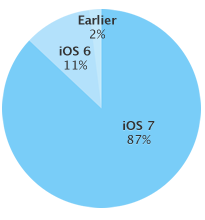
\includegraphics{img/ios7stats}
		\caption{Graf verzí iOS k 27.4.2014}\label{graph:ios7_stats}
	\end{figure}

\section{Podobné aplikace}\label{sec:competition}

	V rámci analýzy požadavků bylo nutné prozkoumat, zda existují podobné aplikace. Následně v nalezených aplikacích bylo potřeba identifikovat jejich kladné, ale i záporné vlastnosti. Takto získané informace byly následně využity pro zlepšení navrhnované aplikace.

	Analýza podobných aplikací byla zaměřena především na uživatelské rozhraní nalezených aplikací a funkce, které aplikace nabízí. U funkcí bylo důležitým kritériem, zda jsou užitečné pro florbalové trenéry.

	\subsection{CoachNote Hockey And Ringette}

	Tato aplikace\footnote{v době analýzy byla dostupná verze 1.6.6} se od začátku analýzy jevila jako nejkvalitnější ze všech nalezených. Zároveň se svým zaměřením i nabízenou funkcionalitou zaměřovala na podobnou cílovou skupinu uživatelů jako aplikace navrhovaná v této práci.

	\begin{figure}[h!]
		\centering
		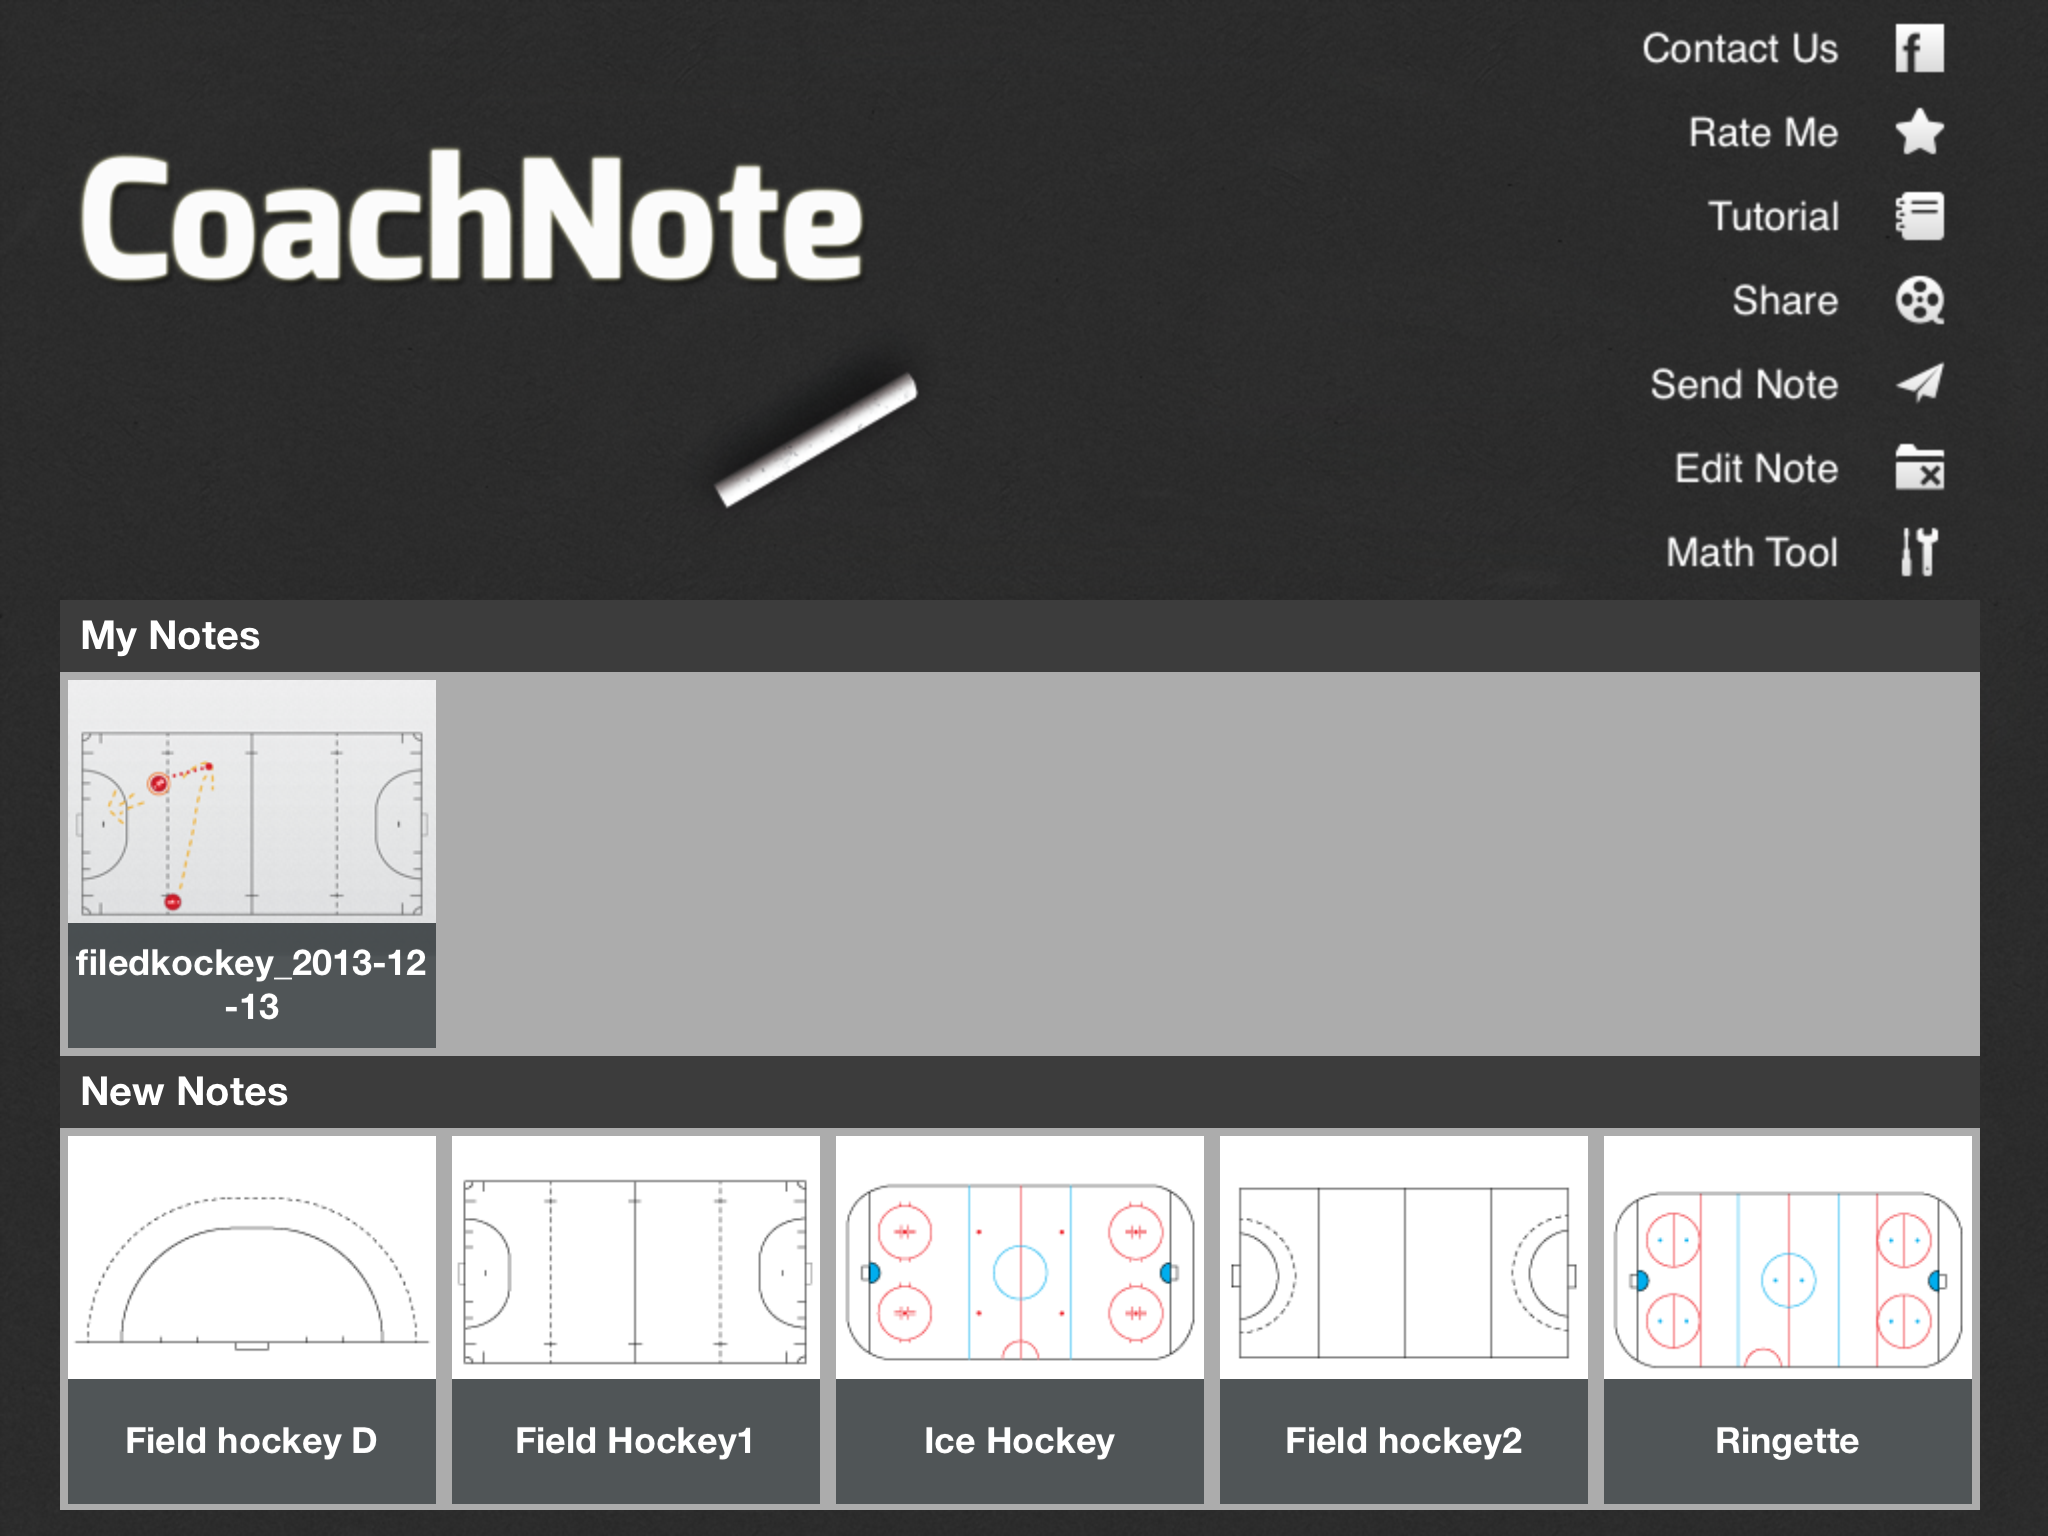
\includegraphics[width=\textwidth]{img/competition/coachnote/IMG_0015}
		\caption{Hlavní menu aplikace CoachNote Hockey And Ringette}
		\label{pic:coachnote_menu}
	\end{figure}

	Uživatelské rozhraní (obr. \ref{pic:coachnote_menu} a \ref{pic:coachnote_exercises}) vypadá podle mého názoru líbivě, nicméně toto je vykoupeno jeho nižší intuitivitou. Aplikace nabízí velké množství funkcí, které je občas složité dohledat. Zároveň ikony, které byly zvoleny pro nástroje mohou uživatele zmást (např. ikona pro skrytí panelu nahrávaní zvuku).

	Rozšířené možnosti jednotlivých nástrojů jsou dostupné po druhém tapnutí na zvolený nástroj. Toto řešení považuji za nešťastné, jelikož jiné kreslicí nástroje, nejen na platformě iOS, řeší tyto věci jiným způsobem, např. změnou položek ve speciálním panelu, který je pro rozšířená nastavení zvoleného nástroje určen. Z tohoto důvodu si myslím, že uživatel často rozšířené možnosti nástroje nenajde.

	\begin{figure}[h!]
		\centering
		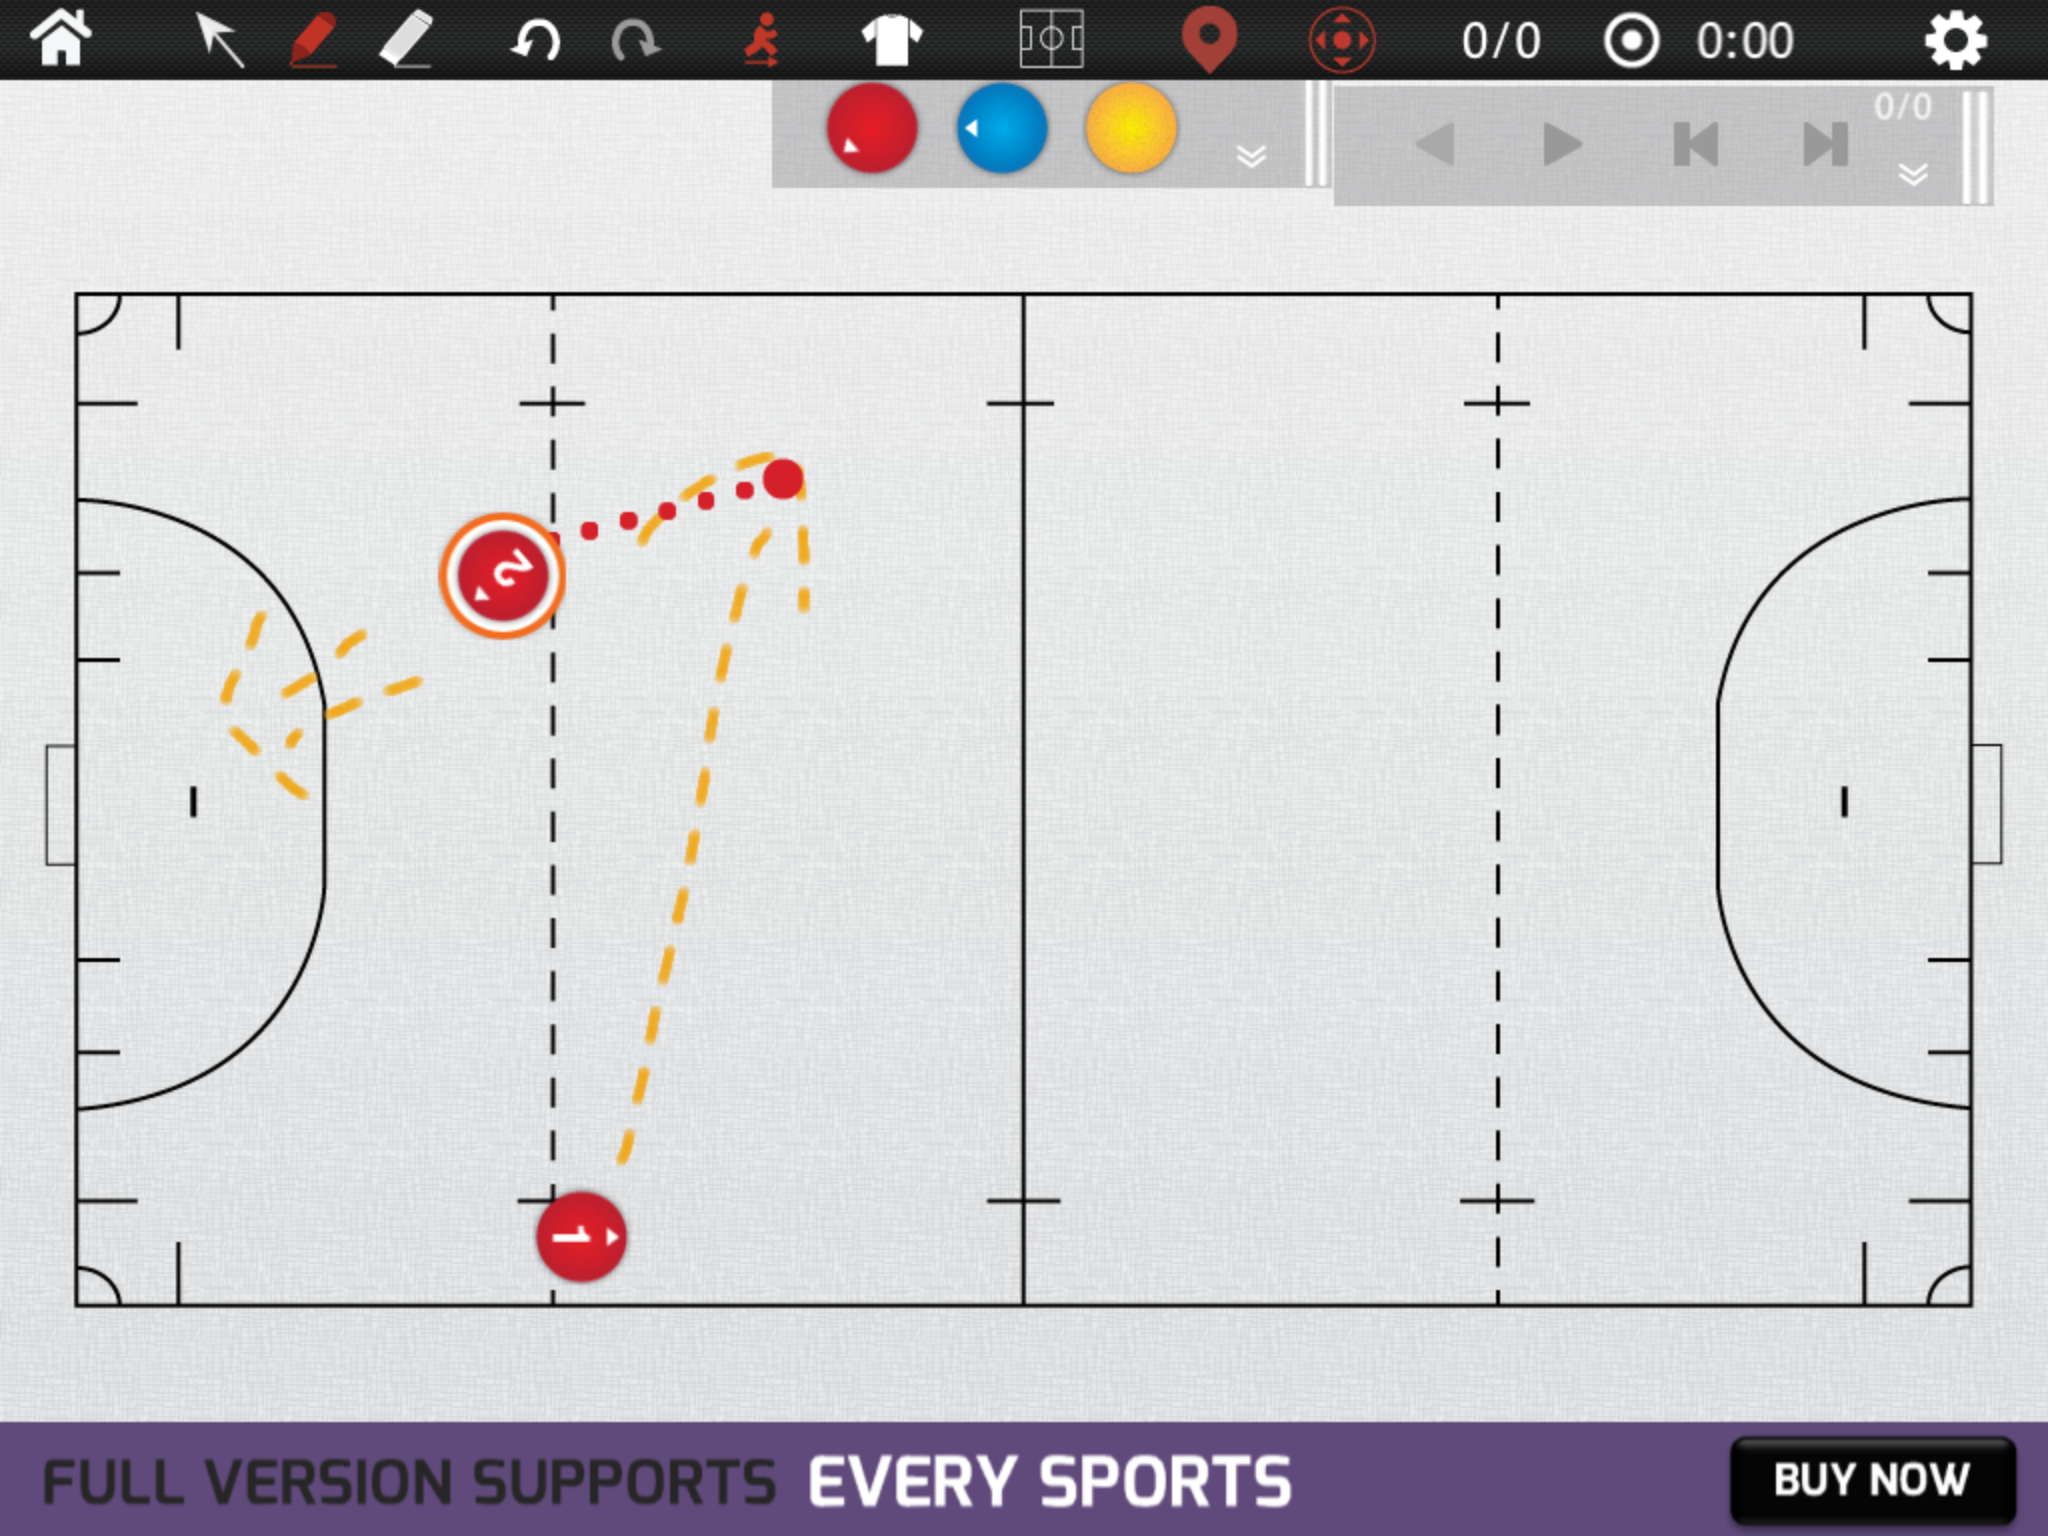
\includegraphics[width=\textwidth]{img/competition/coachnote/IMG_0011}
		\caption{Zobrazení cvičení v aplikaci CoachNote Hockey And Ringette}
		\label{pic:coachnote_exercises}
	\end{figure}

	Po stránce dostupných funkcí by aplikace florbalovému trenérovi mohla vyhovovat. Nicméně pro zobrazení hráčů využívá jinou notaci \-- odlišuje je pouze pomocí barev, což je mezi florbalovými trenéry podle mého názoru nedostačující, protože trenéři i hráči jsou zvyklí rozlišení pomocí různých symbolů.

	U aplikace je šikovné, že hráči jsou speciální objekty, které je možné přesouvat a aplikace zobrazuje jejich trajektorii. Bohužel tato funkce není dotažená do konce a hráče lze přesunout pouze z bodu A do bodu B, pokud je potřeba jej přesunout do dalšího bodu, pak jeho předchozí trajektorie zmizí.

	Aplikace obsahuje velké množství funkcí, některé jsou podle mého názoru zbytečné (např. nahrávání zvuku) a jiné důležité chybí. Jednou z takových funkcí, kterou se mi nepodařilo dohledat je mazání jednotlivých hráčů. Aplikace nabízí pouze možnost smazat všechny hráče, kteří jsou na hřišti zakresleni, což považuji za velký nedostatek, obzvlášť pokud uvažujeme, jak je aplikace komplexní.

	Analýza této aplikace byla zaměřena především na verzi, která je dostupná zdarma na \href{https://itunes.apple.com/us/app/coachnote-hockey-ringette/id562205341?mt=8}{App store}. Placená verze aplikace je osvobozena od reklamy a obsahuje rozšířenou funkcionalitu (např. možnost psát text přímo do cvičení).

	Aplikace podporuje i zařízení iPhone, nicméně na tomto zařízení aplikace zkoušena nebyla, poněvadž navrhovaná aplikace se zaměřuje pouze na iPad.

	Existují různé varianty aplikace, které jsou zaměřené na jiné sporty. Ostatní varianty nebyly testovány, protože sporty, na které byly zaměřeny se od florbalu významně liší.

	Aplikace celkově není špatné, při doplnění florbalové notace a po úpravě uživatelského rozhraní by mohla být dobře použitelná. Co by mohlo být pro uživatele nepříjemné, je až příliš dlouhé čekání při otevření prázdného cvičení\footnote{vyzkoušeno na iPadu 4 a na iPadu Air}.

	\subsection{IceHockey Board Free}

	Aplikace \footnote{v době analýzy byla dostupná verze 8.4} je zdarma dostupná na \href{https://itunes.apple.com/ca/app/icehockey-board-free/id366079177?mt=8}{App store}. Aplikace je zaměřena na lední hokej, existují varianty pro jiné sporty, např. pozemní hokej, ale varianta pro florbal chybí.

	Aplikace je velmi jednoduchá, obsahuje pevný počet hráčů (6 pro každý z týmů). Aplikace si umí ukládat pozice hráčů a poté mezi těmito uloženými stavy lze tapnutím přecházet. Toto platí pouze pro pozice hráčů, nakreslené čáry jsou zobrazeny vždy, bez ohledu na uložený stav.

	Uživatelské rozhraní (obr. \ref{pic:icehockey_board_free}) v aplikaci je minimalistické, po spuštění se zobrazí hřiště a lze s ním ihned manipulovat. Jednotlivé nástroje jsou dostupné po rozvinutí pomocného panelu, který je naznačen vhodnou ikonou.

	\begin{figure}[p]
		\centering
		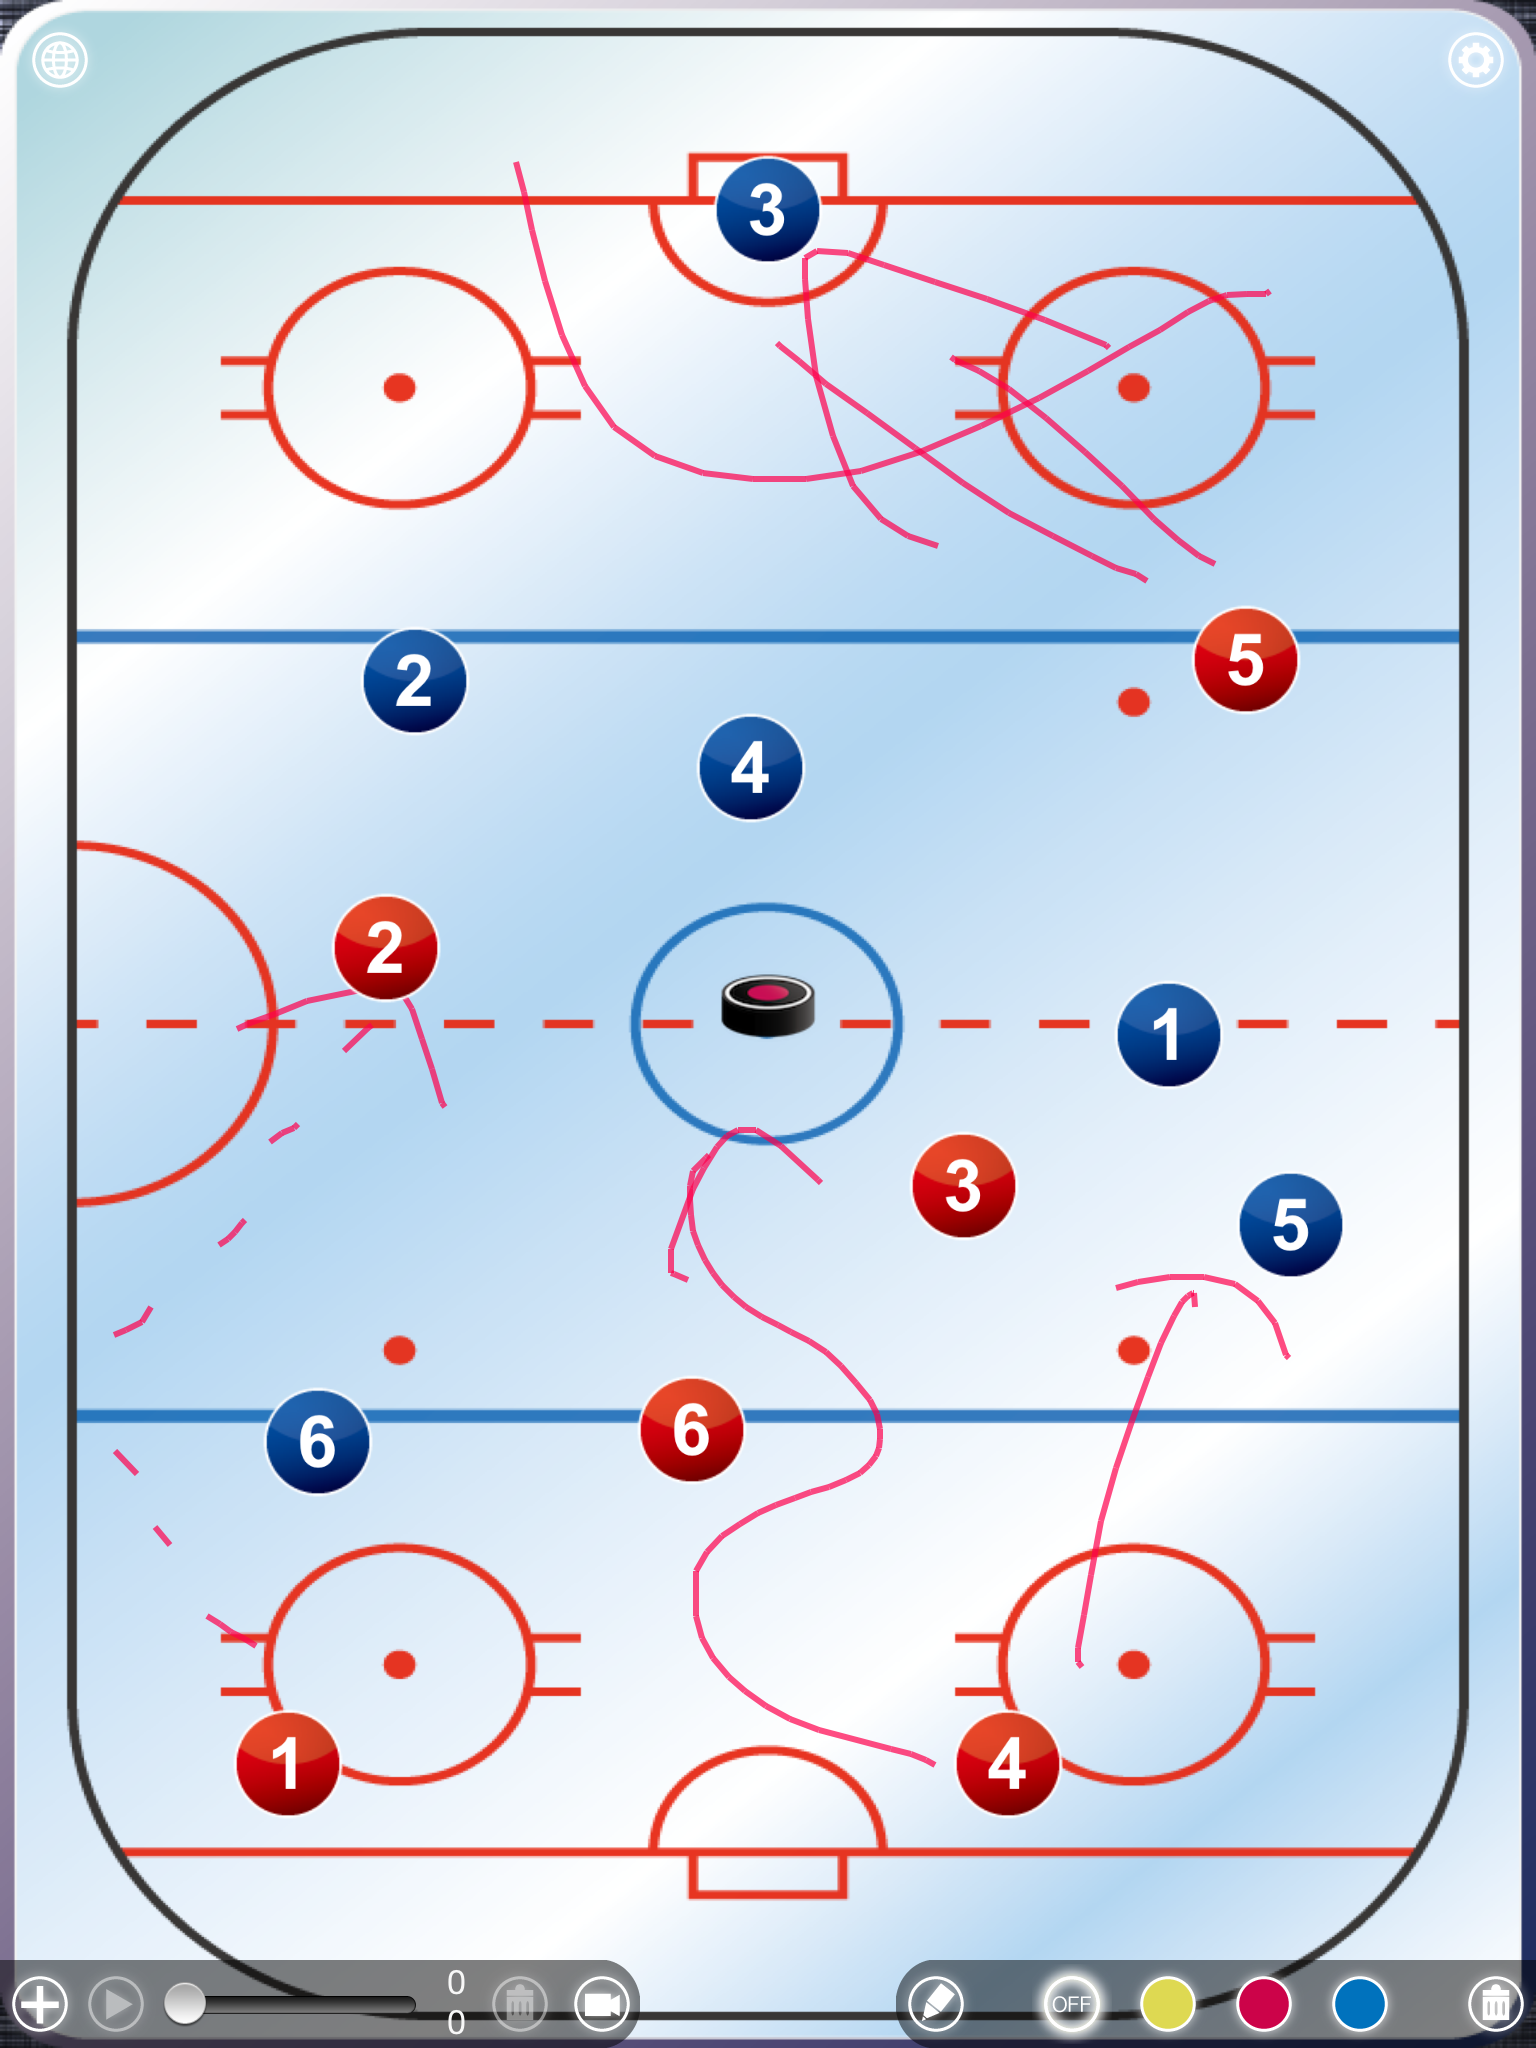
\includegraphics[width=\textwidth]{img/competition/icehockey_board_free/IMG_0018}
		\caption{Uživatelské rozhraní aplikace IceHockey Board Free}
		\label{pic:icehockey_board_free}
	\end{figure}

	Po funkční stránce je aplikace příliš jednoduchá, neumožňuje mazání jednotlivých čar, mazat lze pouze všechny čáry hromadně. Na aplikaci je hezké, že umožňuje automatické nakreslení cvičení, avšak tato funkcionalita není dotažena a týká se pouze pozic jednotlivých hráčů. Tato aplikace posloužila pouze jako příklad, jak by navrhovaná aplikace neměla vypadat, rozhraní není pro uživatele přívětivé a funkce jsou omezené a nedotažené. Dále aplikace obsahuje pro uživatele velmi nepříjemnou reklamu, která jej zdržuje od užívání při spuštění a při každé maximalizaci aplikace.

	\newpage

	\subsection{My Field Hockey Coach Free}

	Verze aplikace\footnote{v době analýzy byla dostupná verze 3.1}, která je dostupná zdarma na \href{https://itunes.apple.com/us/app/my-field-hockey-coach-free/id457826679?mt=8}{App store} je velice omezená, je zaměřená na pozemní hokej. Umožňuje pouze správu jednotlivých hráčů v týmu a jejich rozmístění do formace. Další funkce této aplikace neodpovídají zaměření navrhované aplikace \-- jedná se o možnost zobrazení ukazatele aktuálního skóre utkání a tabule složící k signalizaci střídání. Aplikace neumožňuje žádnou formu kreslení. Toto by mohlo být obsahem placené verze.

	\begin{figure}[h!]
		\centering
		\subfloat[Hlavní nabídka]{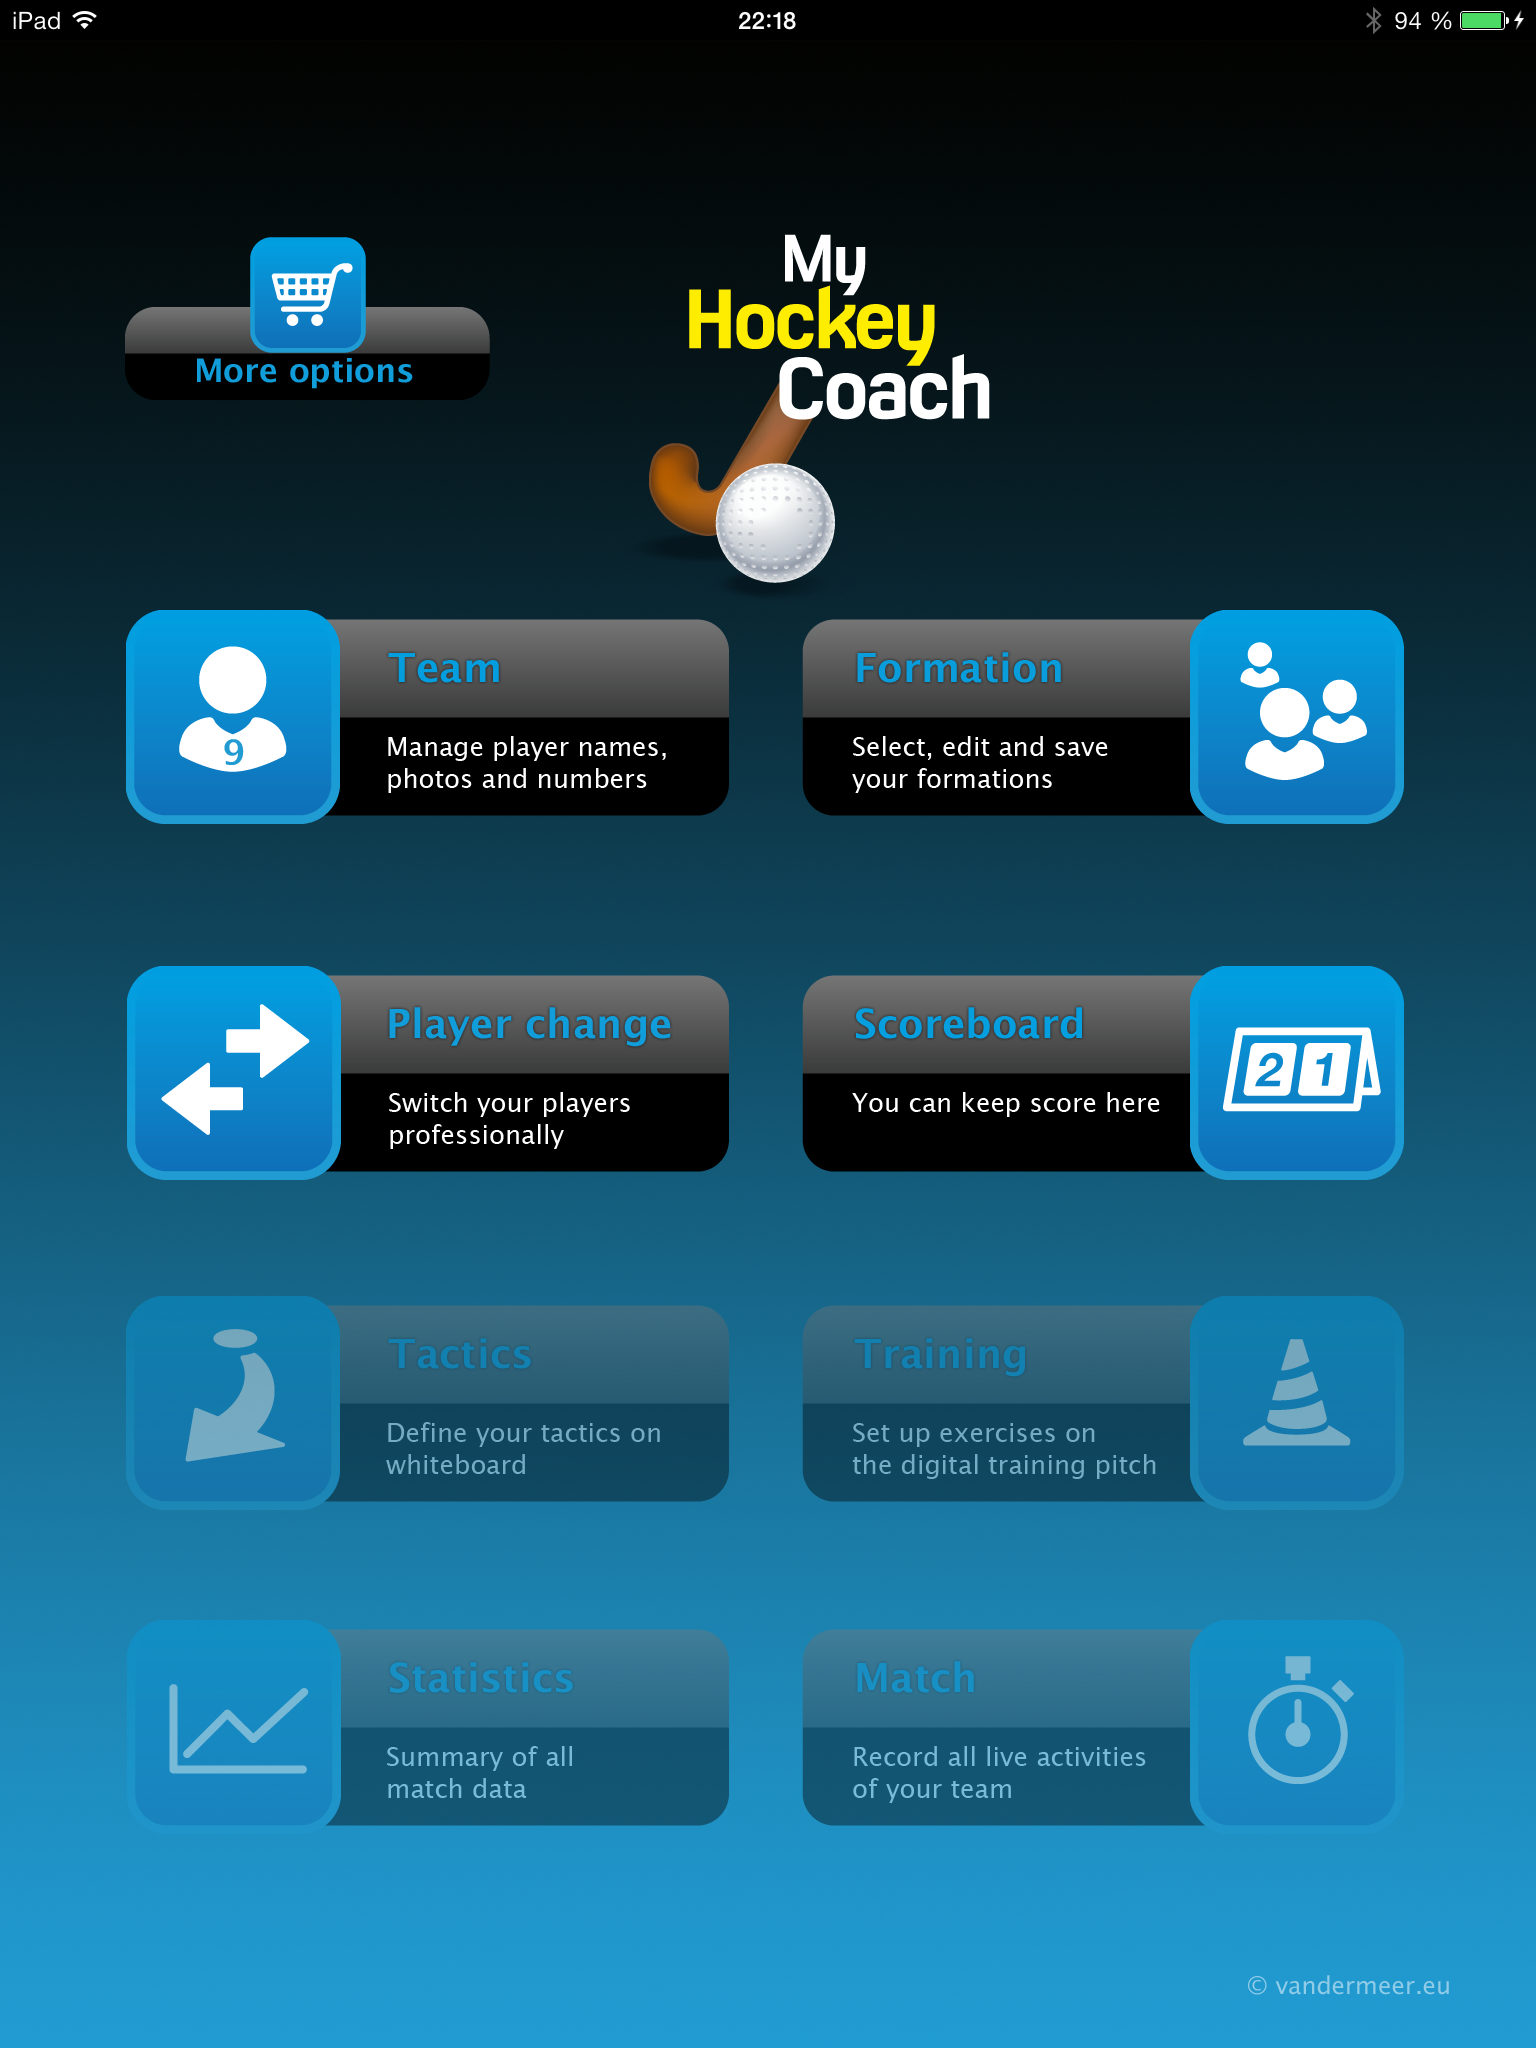
\includegraphics[width=0.4\textwidth]{img/competition/my_field_hockey_coach_free/IMG_0019}}
 		\hfil
 		\subfloat[Správa hráčů]{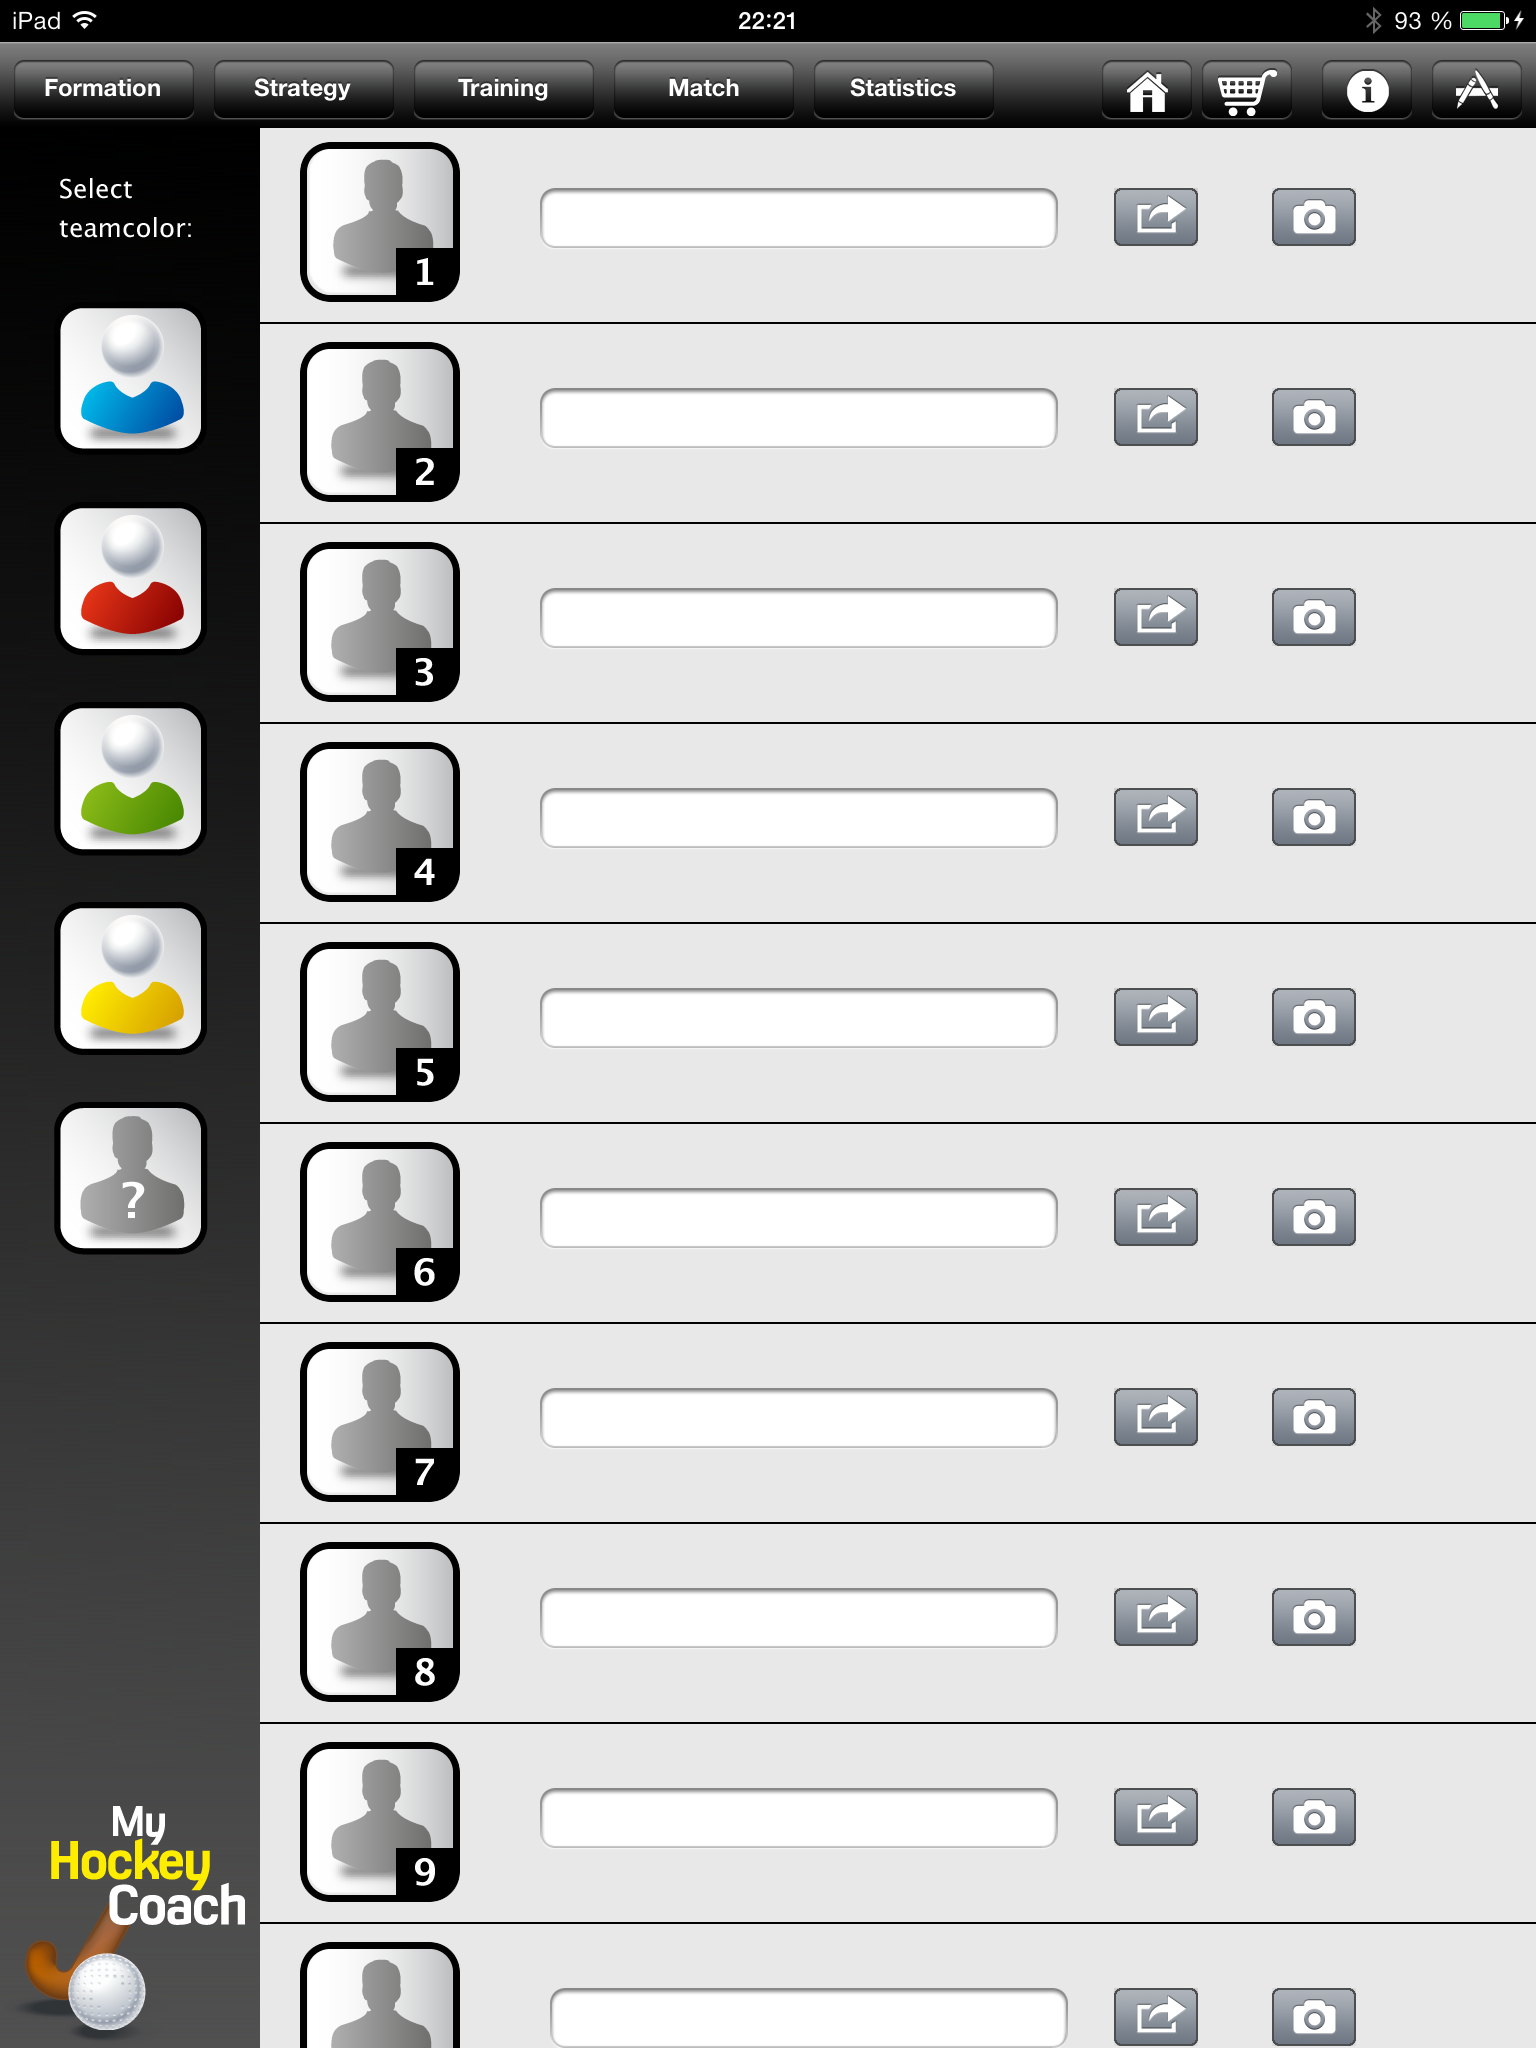
\includegraphics[width=0.4\textwidth]{img/competition/my_field_hockey_coach_free/IMG_0021}}

 		\caption{Uživatelské rozhraní aplikace My Field Hockey Coach Free}
 		\label{pic:my_field_hockey_coach_free}
	\end{figure}

	Aplikace má povedené uživatelské rozhraní (obr. \ref{pic:my_field_hockey_coach_free}. Často jsou pro tlačítka použity textové popisky, čímž je možné se vyvarovat použití matoucí ikony.

	Bylo by dobré se inspirovat návrhem jednotlivých nabídek v menu, které jsou navrženy přehledně a intuitivně. Naopak rozhraní pro kreslicí ploch v aplikaci chybí, tudíž jej nelze jakkoliv analyzovat.

	\subsection{Exercise drawer}

	Aplikace psaná v Javě, tudíž běžící na desktopových platformách, volně dostupná na \href{http://floorballcoach.org/exercisedrawer/}{internetu}. Jedná se o aplikaci, která byla zmíněna v dotazníkovém šetření (kapitola \ref{sec:survey}). Aplikaci považuji vhodnou na přípravu materiálů, pokud autor chce např. publikovat knížku o trénování.

	Funkcemi se aplikace velmi podobá aplikaci navrhované v této práci. Jako jediná je zaměřena na florbal. Nicméně některé funkce jsou omezené, např. je možné kreslit pouze úsečky \-- funkce volného kreslení chybí. Aplikace neumožňuje přípravu celých tréninků, je možné ukládat cvičení pouze jednotlivě. Je možné ke cvičení vkládat poznámky a to dvojím způsobem. Prvním je možnost vkládat poznámky přímo na plochu cvičení, druhá je možnost připsat právě jednu poznámku a uložit ji jako přílohu ke cvičení.

	Aplikace dále umí zobrazit mnoho typů hřiště, nicméně všechny typy jsou pouze mírně obměněné varianty nákresu celého hřiště a poloviny hřiště.

	Po funkční stránce mě zklamalo, že v aplikaci nelze, popř. není snadné, smazat nakreslenou přihrávku, střelu ani pohyb hráče. Bylo možné smazat pouze hráče či kužel.

	\begin{figure}[h!]
		\centering
		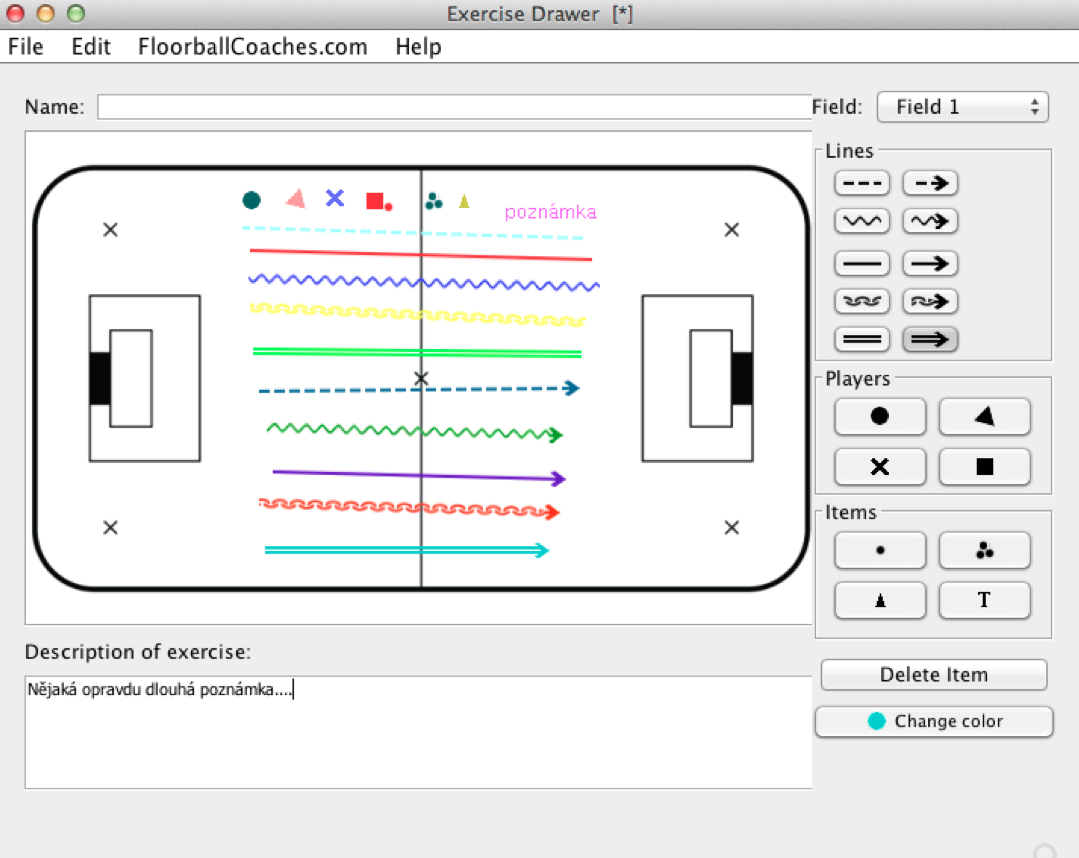
\includegraphics[width=\textwidth]{img/competition/exercise_drawer}
		\caption{Uživatelské rozhraní aplikace Exercise Drawer}
		\label{pic:exercise_drawer}
	\end{figure}

	Uživatelské rozhraní aplikace (obr. \ref{pic:exercise_drawer}) je jednoduché a přehledné, což připisuji především zvolené platformě a velikosti monitoru, na kterém byla aplikace zkoušena.

	Tato aplikace je co se týče funkční stránky pravděpodobně nejlepší a bylo by dobré, aby navrhovaná aplikace byla jejím ekvivalentem na platformě iOS.

	\subsection{Aplikace zmíněné v dotaznících}

	V provedeném dotazníkovém šetření \ref{sec:survey} byly zmíněny ještě další aplikace \-- Florbalový trenér a CoachAp (obě pro OS Android), nicméně ani jednu nebylo možné na Google Play Store nalézt, tudíž nebyly analyzovány.

\section{Návrh uživatelského rozhraní}

\chapter{Realizace}

\section{Architektura aplikace}

\section{Uživatelské rozhraní}

\chapter{Testování}

\begin{conclusion}
	%sem napište závěr Vaší práce
\end{conclusion}

\bibliographystyle{csn690}
\bibliography{mybibliographyfile}

\appendix

\chapter{Seznam použitých zkratek}
% \printglossaries
\begin{description}
	\item[GUI] Graphical user interface
	\item[XML] Extensible markup language
\end{description}


% % % % % % % % % % % % % % % % % % % % % % % % % % % %
% % Tuto kapitolu z výsledné práce ODSTRAŇTE.
% % % % % % % % % % % % % % % % % % % % % % % % % % % %
%
% \chapter{Návod k~použití této šablony}
%
% Tento dokument slouží jako základ pro napsání závěrečné práce na Fakultě informačních technologií ČVUT v~Praze.
%
% \section{Výběr základu}
%
% Vyberte si šablonu podle druhu práce (bakalářská, diplomová), jazyka (čeština, angličtina) a kódování (ASCII, \mbox{UTF-8}, \mbox{ISO-8859-2} neboli latin2 a nebo \mbox{Windows-1250}).
%
% V~české variantě naleznete šablony v~souborech pojmenovaných ve formátu práce\_kódování.tex. Typ může být:
% \begin{description}
% 	\item[BP] bakalářská práce,
% 	\item[DP] diplomová (magisterská) práce.
% \end{description}
% Kódování, ve kterém chcete psát, může být:
% \begin{description}
% 	\item[UTF-8] kódování Unicode,
% 	\item[ISO-8859-2] latin2,
% 	\item[Windows-1250] znaková sada 1250 Windows.
% \end{description}
% V~případě nejistoty ohledně kódování doporučujeme následující postup:
% \begin{enumerate}
% 	\item Otevřete šablony pro kódování UTF-8 v~editoru prostého textu, který chcete pro psaní práce použít -- pokud můžete texty s~diakritikou normálně přečíst, použijte tuto šablonu.
% 	\item V~opačném případě postupujte dále podle toho, jaký operační systém používáte:
% 	\begin{itemize}
% 		\item v~případě Windows použijte šablonu pro kódování \mbox{Windows-1250},
% 		\item jinak zkuste použít šablonu pro kódování \mbox{ISO-8859-2}.
% 	\end{itemize}
% \end{enumerate}
%
%
% V~anglické variantě jsou šablony pojmenované podle typu práce, možnosti jsou:
% \begin{description}
% 	\item[bachelors] bakalářská práce,
% 	\item[masters] diplomová (magisterská) práce.
% \end{description}
%
% \section{Použití šablony}
%
% Šablona je určena pro zpracování systémem \LaTeXe{}. Text je možné psát v~textovém editoru jako prostý text, lze však také využít specializovaný editor pro \LaTeX{}, např. Kile.
%
% Pro získání tisknutelného výstupu z~takto vytvořeného souboru použijte příkaz \verb|pdflatex|, kterému předáte cestu k~souboru jako parametr. Vhodný editor pro \LaTeX{} toto udělá za Vás. \verb|pdfcslatex| ani \verb|cslatex| \emph{nebudou} s~těmito šablonami fungovat.
%
% Více informací o~použití systému \LaTeX{} najdete např. v~\cite{wikilatex}.
%
% \subsection{Typografie}
%
% Při psaní dodržujte typografické konvence zvoleného jazyka. České \uv{uvozovky} zapisujte použitím příkazu \verb|\uv|, kterému v~parametru předáte text, jenž má být v~uvozovkách. Anglické otevírací uvozovky se v~\LaTeX{}u zadávají jako dva zpětné apostrofy, uzavírací uvozovky jako dva apostrofy. Často chybně uváděný symbol "{} (palce) nemá s~uvozovkami nic společného.
%
% Dále je třeba zabránit zalomení řádky mezi některými slovy, v~češtině např. za jednopísmennými předložkami a spojkami (vyjma \uv{a}). To docílíte vložením pružné nezalomitelné mezery -- znakem \texttt{\textasciitilde}. V~tomto případě to není třeba dělat ručně, lze použít program \verb|vlna|.
%
% Více o~typografii viz \cite{kobltypo}.
%
% \subsection{Obrázky}
%
% Pro umožnění vkládání obrázků je vhodné použít balíček \verb|graphicx|, samotné vložení se provede příkazem \verb|\includegraphics|. Takto je možné vkládat obrázky ve formátu PDF, PNG a JPEG jestliže používáte pdf\LaTeX{} nebo ve formátu EPS jestliže používáte \LaTeX{}. Doporučujeme preferovat vektorové obrázky před rastrovými (vyjma fotografií).
%
% \subsubsection{Získání vhodného formátu}
%
% Pro získání vektorových formátů PDF nebo EPS z~jiných lze použít některý z~vektorových grafických editorů. Pro převod rastrového obrázku na vektorový lze použít rasterizaci, kterou mnohé editory zvládají (např. Inkscape). Pro konverze lze použít též nástroje pro dávkové zpracování běžně dodávané s~\LaTeX{}em, např. \verb|epstopdf|.
%
% \subsubsection{Plovoucí prostředí}
%
% Příkazem \verb|\includegraphics| lze obrázky vkládat přímo, doporučujeme však použít plovoucí prostředí, konkrétně \verb|figure|. Například obrázek \ref{fig:float} byl vložen tímto způsobem. Vůbec přitom nevadí, když je obrázek umístěn jinde, než bylo původně zamýšleno -- je tomu tak hlavně kvůli dodržení typografických konvencí. Namísto vynucování konkrétní pozice obrázku doporučujeme používat odkazování z~textu (dvojice příkazů \verb|\label| a \verb|\ref|).
%
% \begin{figure}\centering
% 	
\includegraphics[width=0.5\textwidth, angle=30]{cvut-logo-bw}
% 	\caption[Příklad obrázku]{Ukázkový obrázek v~plovoucím prostředí}\label{fig:float}
% \end{figure}
%
% \subsubsection{Verze obrázků}
%
% % Gnuplot BW i barevně
% Může se hodit mít více verzí stejného obrázku, např. pro barevný či černobílý tisk a nebo pro prezentaci. S~pomocí některých nástrojů na generování grafiky je to snadné.
%
% Máte-li například graf vytvořený v programu Gnuplot, můžete jeho černobílou variantu (viz obr. \ref{fig:gnuplot-bw}) vytvořit parametrem \verb|monochrome dashed| příkazu \verb|set term|. Barevnou variantu (viz obr. \ref{fig:gnuplot-col}) vhodnou na prezentace lze vytvořit parametrem \verb|colour solid|.
%
% \begin{figure}\centering
% 	\includegraphics{gnuplot-bw}
% 	\caption{Černobílá varianta obrázku generovaného programem Gnuplot}\label{fig:gnuplot-bw}
% \end{figure}
%
% \begin{figure}\centering
% 	\includegraphics{gnuplot-col}
% 	\caption{Barevná varianta obrázku generovaného programem Gnuplot}\label{fig:gnuplot-col}
% \end{figure}
%
%
% \subsection{Tabulky}
%
% Tabulky lze zadávat různě, např. v~prostředí \verb|tabular|, avšak pro jejich vkládání platí to samé, co pro obrázky -- použijte plovoucí prostředí, v~tomto případě \verb|table|. Například tabulka \ref{tab:matematika} byla vložena tímto způsobem.
%
% \begin{table}\centering
% 	\caption[Příklad tabulky]{Zadávání matematiky}\label{tab:matematika}
% 	\begin{tabular}{|l|l|c|c|}\hline
% 		Typ		& Prostředí		& \LaTeX{}ovská zkratka	& \TeX{}ovská zkratka	\tabularnewline \hline \hline
% 		Text		& \verb|math|		& \verb|\(...\)|	& \verb|$...$|		\tabularnewline \hline
% 		Displayed	& \verb|displaymath|	& \verb|\[...\]|	& \verb|$$...$$|	\tabularnewline \hline
% 	\end{tabular}
% \end{table}
%
% % % % % % % % % % % % % % % % % % % % % % % % % % % %

\chapter{Obsah přiloženého CD}

%upravte podle skutecnosti

\begin{figure}
	\dirtree{%
		.1 readme.txt\DTcomment{stručný popis obsahu CD}.
		.1 exe\DTcomment{adresář se spustitelnou formou implementace}.
		.1 src.
		.2 impl\DTcomment{zdrojové kódy implementace}.
		.2 thesis\DTcomment{zdrojová forma práce ve formátu \LaTeX{}}.
		.1 text\DTcomment{text práce}.
		.2 thesis.pdf\DTcomment{text práce ve formátu PDF}.
		.2 thesis.ps\DTcomment{text práce ve formátu PS}.
	}
\end{figure}

\end{document}
